\documentclass{article}
\usepackage{aistats2018}
% Camera ready: \usepackage[accepted]{aistats2018}
\newif\ifanonymized
\anonymizedtrue
% Camera ready: \anonymizedfalse

\usepackage[round]{natbib}
\usepackage[utf8]{inputenc} % allow utf-8 input
\usepackage[T1]{fontenc}    % use 8-bit T1 fonts
\usepackage{lmodern}
\usepackage[hidelinks]{hyperref}       % hyperlinks
\usepackage{url}            % simple URL typesetting
\usepackage{booktabs}       % professional-quality tables
\usepackage{amsfonts}       % blackboard math symbols
\usepackage{nicefrac}       % compact symbols for 1/2, etc.
\usepackage{microtype}      % microtypography
\usepackage{graphicx}
\usepackage{algorithm}% http://ctan.org/pkg/algorithms
\usepackage{algpseudocode}% http://ctan.org/pkg/algorithmicx
\usepackage{booktabs}


\usepackage{amsmath}
\usepackage{amssymb}
\usepackage{amsfonts}
%\usepackage{enumerate}
%\usepackage{bbm}
%\usepackage{caption}

\newcommand{\pa}[1]{ \left({#1}\right) }

\def \N {\mathbb{N}}
\def \Nbr {\mathcal{N}}
\def \Q {\mathbb{Q}}
\def \F {\mathbb{F}}
\def \then {\implies &}
\def \oif {\Longleftrightarrow &\,}
\def \given {\text{Given }&}
\def \assume {\text{Assume }&}
\def \thfr {\therefore &\enskip}
\def \bij {\leftrightarrow}
\def \inj {\rightarrowtail}
\def \sur {\twoheadedrightarrow}
\def \Z {\mathbb{Z}}
\def \R {\mathbb{R}}
\def \C {\mathbb{C}}
\def \T {\mathbb{T}}
\def \iff {\Longleftrightarrow}
\def \kron {\boldsymbol\delta}
%\def \indicator {\mathbbm{1}}

\def\tbr{{\textbf{r}}}
\def\Ts{\textbf{s}}
\def\Ta{\textbf{a}}
\def\Tm{\textbf{m}}
\def\Tb{\textbf{b}}
\def\Tc{\textbf{c}}
\def\Td{\textbf{d}}
\def\Te{\textbf{e}}
\def\Tv{\textbf{v}}
\def\Tx{\textbf{x}}
\def\TX{\textbf{X}}
\def\TU{\textbf{U}}
\def\Tu{\textbf{u}}
\def\Ty{\textbf{y}}
\def\Tk{\textbf{k}}
\def\Tt{\textbf{t}}
\def\Tz{\textbf{z}}
\def\quotient{\mathclose{}/\mathopen{}}
\def\Tf{\textbf{f}}
\def\Th{\textbf{h}}
\def\Tg{\textbf{g}}
\def\sumn{\sum_{n=0}^\infty}
\def\limn{\lim_{n\rightarrow\infty}}
\def\prodn{\prod_{n=0}^\infty}

\def\bsz{\textbf{0}}
\def\bs1{\textbf{1}}
\def\bsa{{\boldsymbol\alpha}}
\def\bse{{\boldsymbol\eta}}
\def \bss{ {\boldsymbol\sigma}}

\DeclareMathOperator{\conv}{conv}
\DeclareMathOperator\cat{cat}
\DeclareMathOperator\adj{adj}
\DeclareMathOperator\Pois{Pois}
\DeclareMathOperator\Id{Id}
\DeclareMathOperator\mathProb{\mathbb{P}}
\def\P{\mathProb} % need to overwrite stupid paragraph symbol
\DeclareMathOperator\mathExp{\mathbb{E}}
\def \E {\mathExp}


\newcommand{\stc}[1]{\widetilde{#1}}   
\newcommand{\set}[2]{ \left\{ #1 \,\middle|\, #2 \right\} }
\newcommand{\idx}[3]{ \left\{ #1 \right\}_{ #2 }^{ #3 } }
\newcommand{\shift}[1]{&\quad & \text{#1}\\}
\newcommand{\lem}[1]{\text{\textbf{L.\ref{#1}}}}
\newcommand{\card}[1]{\left\vert{#1}\right\vert}
\newcommand{\colv}[1]{\begin{pmatrix} #1 \end{pmatrix}}
\newcommand{\mat}[1]{\begin{pmatrix} #1 \end{pmatrix}}
\newcommand{\detmat}[1]{\begin{vmatrix} #1 \end{vmatrix}}
\newcommand{\spanb}[1]{\text{span}\{ #1 \}}
\newcommand{\abs}[1]{\left|#1\right|}
\newcommand{\opcat}[1]{#1^{\text{op}}}
\newcommand{\Inner}[1]{\left\langle #1 \right\rangle}
\newcommand{\Innercpy}[1]{\Inner{ #1, #1 }}
\newcommand{\norm}[1]{\left\| #1 \right\|}% use instead of $\|x\|$

\def\eqd{\mathrel{\overset{\Delta}{=}}}

\DeclareMathOperator{\diag}{diag}
\DeclareMathOperator{\vcdim}{VC-dim}
\DeclareMathOperator*{\Err}{\text{err}}
\DeclareMathOperator*{\ErrE}{\mathbb{E}}
\DeclareMathOperator{\Tr}{tr}
\DeclareMathOperator{\Dim}{dim}
\DeclareMathOperator{\Rank}{rank}
\DeclareMathOperator*{\argmin}{argmin}
\DeclareMathOperator*{\proj}{proj}
\DeclareMathOperator{\Ker}{ker}
\DeclareMathOperator{\Diam}{diam}
\DeclareMathOperator{\Int}{int}
\DeclareMathOperator{\Clo}{clo}
\DeclareMathOperator{\sgn}{sgn}
\DeclareMathOperator{\MyRe}{Re}
\DeclareMathOperator{\MyIm}{Im}
\DeclareMathOperator{\image}{image}
\DeclareMathOperator{\colim}{colim}
\DeclareMathOperator{\Supp}{supp}
\DeclareMathOperator{\Var}{var}
\DeclareMathOperator{\Hom}{hom}
\DeclareMathOperator{\Ob}{ob}
\DeclareMathOperator{\El}{el}
\DeclareMathOperator\power{{\mathcal{P}}}
\DeclareMathOperator{\Nat}{Nat}
\DeclareMathOperator{\cone}{cone}
\DeclareMathOperator{\vectorize}{vec}
\DeclareMathOperator{\matricize}{mat}
\DeclareMathOperator{\cov}{cov}
\DeclareMathOperator{\Unif}{Unif}
\DeclareMathOperator{\blockdiag}{blockdiag}
\DeclareMathOperator{\mvm}{MVM}

% probability stuff
\def \sa {{$\sigma$-algebra}}
\def\OR{{\overline{\R}}}
\def\OX{{\overline{X}}}

\def\mcU{{\mathcal{U}}}
\def \mcX {\mathcal{X}}
\def \mcS {\mathcal{S}}
\def \mcY {\mathcal{Y}}
\def \mcL {\mathcal{L}}
\def \mcD {\mathcal{D}}
\def \mcC {\mathcal{C}}
\def \mcA {\mathcal{A}}
\def \mcK {\mathcal{K}}
\def \mcM {\mathcal{M}}
\def\mcG{{\mathcal{G}}}
\def\mcH{{\mathcal{H}}}
\def\mcF{{\mathcal{F}}}
\def\mcB{{\mathcal{B}}}
\def\mcE{{\mathcal{E}}}
\def\mcI{{\mathcal{I}}}
\def\mcQ{{\mathcal{Q}}}
\def\mcM{{\mathcal{M}}}
\def\mcC{{\mathcal{C}}}
\def\mcT{{\mathcal{T}}}
\def\mcO{{\mathcal{O}}}
\def\mcJ{{\mathcal{J}}}

\def\bsa{{\boldsymbol\alpha}}
\def\bsr{{\textbf{r}}}
\def\bse{{\boldsymbol\epsilon}}
\def\bsk{{\boldsymbol\kappa}}
\def\bsm{{\boldsymbol\mu}}
\def\bsl{{\boldsymbol\lambda}}
\def\bsph{{\boldsymbol\phi}}
\def\bsth{{\boldsymbol\theta}}

\def\abovestrut#1{\rule[0in]{0in}{#1}\ignorespaces}
\def\belowstrut#1{\rule[-#1]{0in}{#1}\ignorespaces}
\def\abovespace{\abovestrut{0.20in}}
\def\belowspace{\belowstrut{0.10in}}





\begin{document}

\ifanonymized

\twocolumn[
\aistatstitle{Supplementary Material for Large Linear Multi-output Gaussian Process Learning}
\aistatsauthor{ Anonymous Author }
\aistatsaddress{ Anonymous Institution }
]
\else
\twocolumn[
\aistatstitle{Supplementary Material for Large Linear Multi-output Gaussian Process Learning}
\aistatsauthor{   {Vladimir Feinberg} \And {Li-Fang Cheng} \And  {Kai Li} \And {Barbara E Engelhardt} }
\aistatsaddress{ UC Berkeley \And Princeton University \And Princeton University \And Princeton University }
]
\fi


\section{Implementation Details}

LLGP was implemented in Python 3 from the Anaconda, which offered an Intel MKL-linked scipy \citep{scipy}. The code made heavy use of other packages, namely climin \citep{climin}, GPy \citep{gpy}, and paramz \citep{paramz}. Code and benchmarks are available at
\ifanonymized
\texttt{<anonymous repository>}.
\else
\url{https://github.com/vlad17/runlmc}.
\fi

Application of our approach to all replication studies was carried out on a large server in a multiprogramming environment: Ubuntu 16.04.3 LTS with 48 Intel(R) Xeon(R) CPU E5-2670 v3 @ 2.30GHz. All experiments in the main report were allotted up to 16 threads (both for COGP MATLAB computation threads and parallel Monte Carlo in the case of LLGP). All experiments in the supplement (below, Sec.~\ref{empirical-rep}) were allotted only 1 thread each.

\section{Representation evaluation}\label{empirical-rep}

We evaluated the performance of the different kernel representations over various rank and parameterization settings. In particular, we have the following parameters: $n$ total sample size across all outputs, $D$ number of outputs, $Q$ number of kernels $k_q$, $R$ average added rank, $\epsilon$ mean noise, and \texttt{ktype} kernel type. Kernel type is one of \texttt{mat, periodic, rbf, mix} corresponding to Mat\'{e}rn-3/2, standard periodic\footnote{We define the periodic kernel as $k(r) = \exp \left(\frac{-\gamma}{2}\sin^2\frac{\pi r}{T}\right)$.}, and radial basis functions. \texttt{mix} refers to a mix of all three kernels.

For each setting, we randomly sample entries for each $A_q,\bsk_q$, and $\bse$ and the inverse length scale $\gamma$ for each kernel. Then, we investigate the average gradient construction accuracy and speed of LLGP for different settings of $Q,\epsilon$, and \texttt{ktype}.Each kernel's inverse length scales and periods were selected by sampling uniformly in log space from 1 to 10 with $Q$ samples. Next, we construct a random LMC kernel by sampling entries of each $A_q$ from a standard normal distribution truncated to the unit interval, $\bsk_q$ from an inverse gamma with unit shape and scale, and independent noise $\bse$ for every output from an inverse gamma with unit scale and mean $\epsilon$. Inputs and outputs were independently generated from $\Unif[0,1]$ for representation evaluation benchmarking.

As expected from their asymptotic runtime, \textsc{sum}, \textsc{bt}, and \textsc{slfm} representations are complimentary in MVM speed for different configurations of $D,R,Q$---this results in sparse inversion computation that consistently outperforms Cholesky decomposition in runtime (Tab.~\ref{complement}).
For inverting systems, all computations were carried out until the residual $\ell_2$ norm was at most $10^{-4}$.
\begin{table*}[!ht]
  \caption{The runtime in seconds for solving $K\Tx=\Ty$ for a random kernel $K$ constructed as in Sec.~\ref{empirical-rep} using \textsc{minres} for each of the kernel representations. For comparison, the \textsc{chol} representation is wallclock time to compute the Cholesky decomposition of the matrix, which must be constructed, and use this decomposition to invert the system. We averaged over five runs. In every run, we use $n=5000$ simulated data points, $\texttt{mix}$ kernels, and $\epsilon=0.1$.
}
\label{complement}
\begin{center}
  \begin{small}
    
\begin{tabular}{|ccc|cccc|}
  \hline
  \abovespace\belowspace
  $D$ & $R$ & $Q$ & \textsc{cholesky} & \textsc{sum} & \textsc{bt} & \textsc{slfm}\\
\hline
  \abovespace
 $ 2 $ & $ 2 $ & $ 10 $ & $ 40.71 $ & $ 38.13 $ & $ \textbf{7.83} $ & $ 59.53 $ \\ 
 $ 10 $ & $ 1 $ & $ 10 $ & $ 37.69 $ & $ 33.15 $ & $ 16.39 $ & $ \textbf{11.59} $ \\ 
  $ 10 $ & $ 10 $ & $ 1 $ & $ 11.19 $ & $ \textbf{0.784} $ & $ 2.48 $ & $ 1.13 $

  \belowspace \\
  \hline
\end{tabular}

\end{small}
\end{center}
\end{table*}

We next evaluated the accuracy of the gradients for $N=10$ trace samples. Fixing $R=3,n=5000,D=10$, we quantified the accuracy LLGP's $\nabla\mcL$ by comparing against the exact Cholesky approach. The relative error in the gradients is generally low for smooth kernels that induce diagonally dominant covariance matrices (Fig.~\ref{fig:relgrad}). Kernels such as the single Mat\'{e}rn or periodic kernel with noise on the order of $10^{-4}$ lead to less accurate gradients, owing to poor \textsc{minres} convergence in the inversions (Fig.~\ref{fig:rellog}). We showed in the main paper that the stochastic gradients suffice for optimization in practical examples.

\begin{figure*}[!ht]
  \centering
{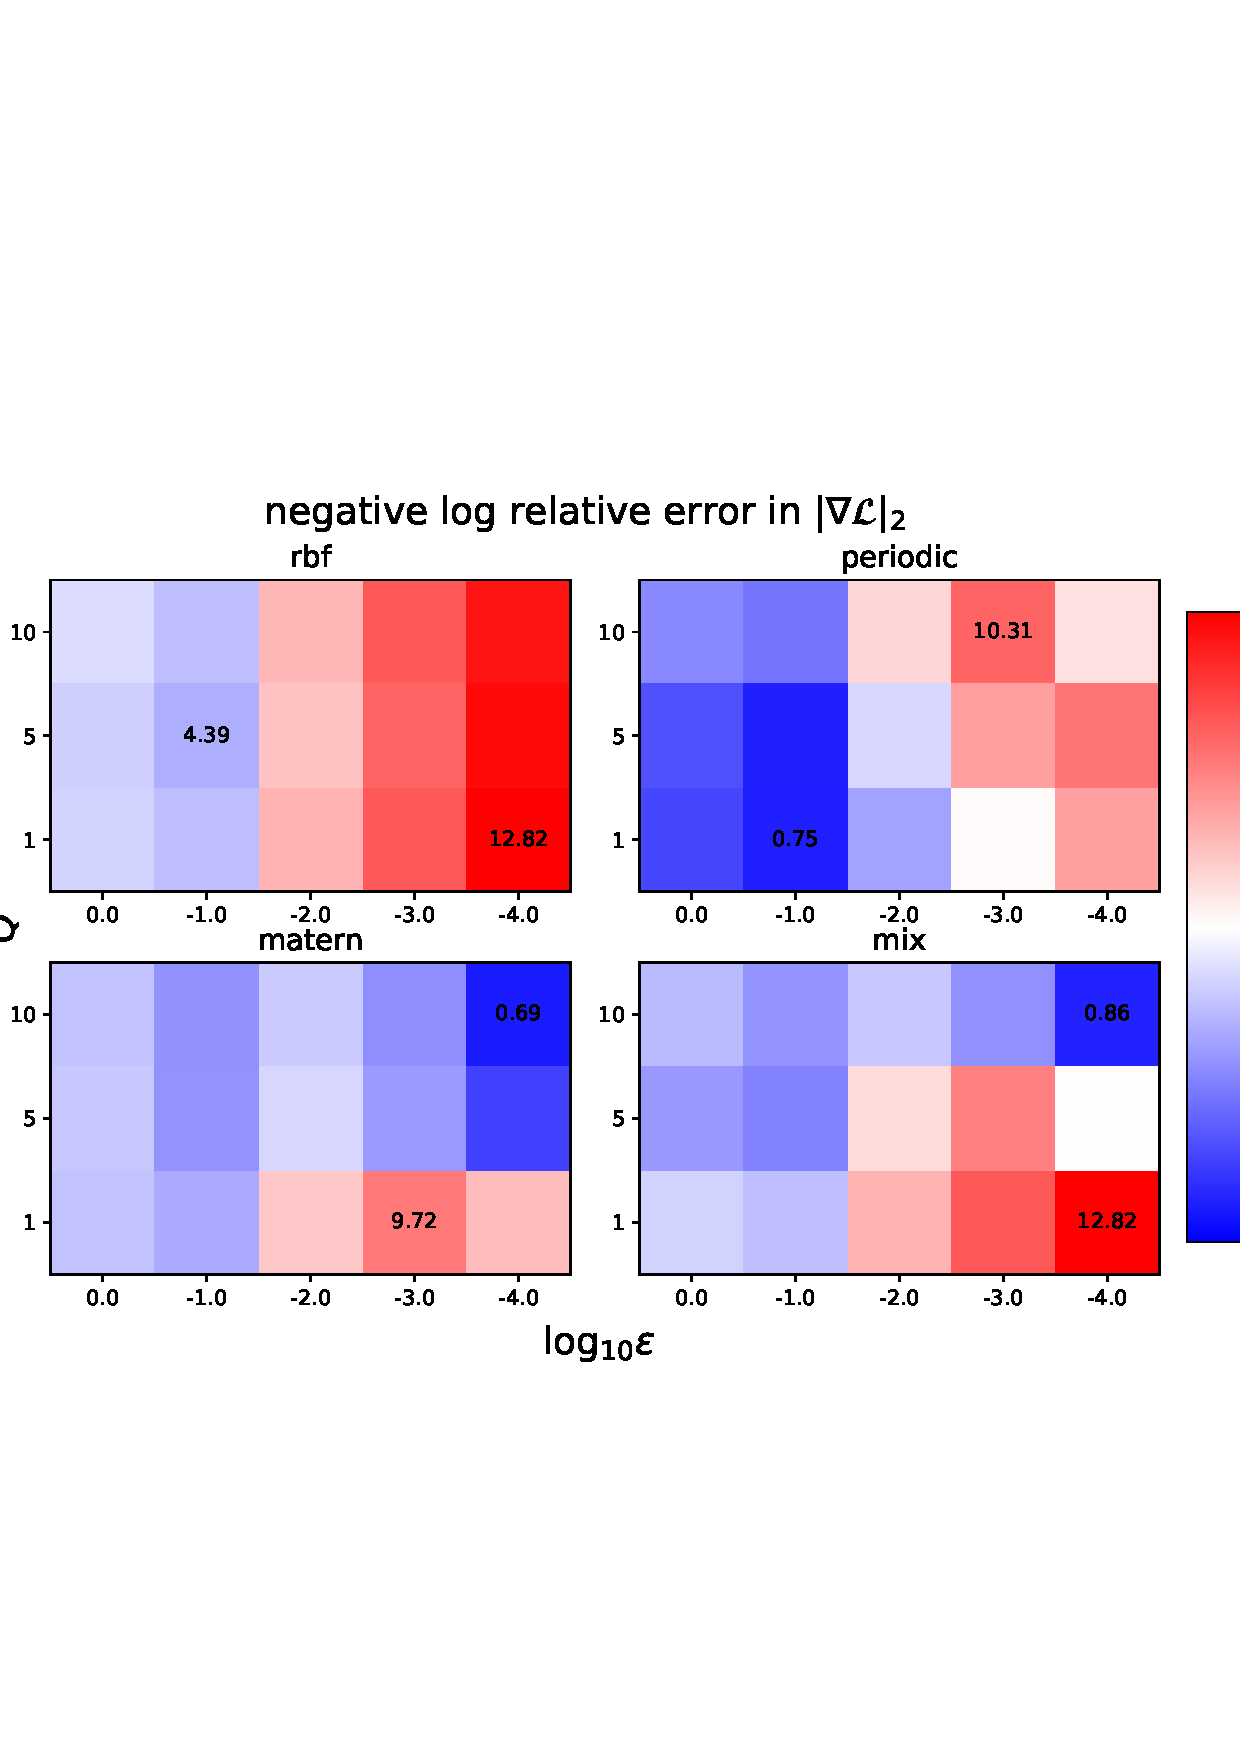
\includegraphics[width=\textwidth]{relgrad_l2.pdf}}
\caption{Negative logarithm of the relative error from the LLGP gradient construction to the exact log likelihood gradient. In each case, higher is better, and extremal values are noted.  For each data point, the average was taken over five runs. Reducing average noise, corresponding to increases in $-\log_{10}\varepsilon$, and increases in $Q$, generally make gradient reconstruction more difficult by making $K$ more ill-conditioned, reducing the accuracy of \textsc{minres}.}
\label{fig:relgrad}
\end{figure*}

\begin{figure*}[!ht]
\centering
{\includegraphics[width=\textwidth]{relalpha_l2.pdf}}
\caption{Negative logarithm of the relative error in $K^{-1}\Ty$, using \textsc{minres} compared to the Cholesky solution. Higher is better, and extremal values are noted. An average was taken over five runs.}
\label{fig:rellog}
\end{figure*}

\bibliographystyle{unsrtnat}
\bibliography{supplement}

\end{document}

